\documentclass[11pt,landscape,a4paper,fleqn]{article}
\usepackage[dvipsnames]{xcolor} 
% https://www.overleaf.com/learn/latex/Using_colours_in_LaTeX#Reference_guide
\usepackage[utf8]{inputenc}
\usepackage[ngerman]{babel}
\usepackage{tikz}
\usetikzlibrary{shapes,positioning,arrows,fit,calc,graphs,graphs.standard}
\usepackage[nosf]{kpfonts}
\usepackage[t1]{sourcesanspro}
%\usepackage[lf]{MyriadPro}
%\usepackage[lf,minionint]{MinionPro}
\usepackage{multicol}
\usepackage{wrapfig}
\usepackage[top=0mm,bottom=3mm,left=1mm,right=1mm]{geometry}
\usepackage[framemethod=tikz]{mdframed}
\usepackage{microtype}
\usepackage{soul}


\let\bar\overline

\definecolor{myblue}{cmyk}{1,.72,0,.38}
% \definecolor{myorange}{cmyk}{0,0.5,1,0}

\pgfdeclarelayer{background}
\pgfsetlayers{background,main}

\everymath\expandafter{\the\everymath \color{myblue}}
\everydisplay\expandafter{\the\everydisplay \color{myblue}}

\renewcommand{\baselinestretch}{.8}
\pagestyle{empty}

\global\mdfdefinestyle{header}{%
linecolor=gray,linewidth=1pt,%
leftmargin=0mm,rightmargin=0mm,skipbelow=0mm,skipabove=0mm,
}

\newcommand{\header}{
\begin{mdframed}[style=header]
\footnotesize
\sffamily
Cheat sheet\\
Ines Pereira,~page~\thepage~of~2
\end{mdframed}
}

\makeatletter
\renewcommand{\section}{\@startsection{section}{1}{0mm}%
                                {.2ex}%
                                {.2ex}%x
                                {\color{Maroon}\sffamily\small\bfseries}}
\renewcommand{\subsection}{\@startsection{subsection}{1}{0mm}%
                                {.2ex}%
                                {.2ex}%x
                                {\color{OliveGreen}\sffamily\bfseries}}
\renewcommand{\subsubsection}{\@startsection{subsubsection}{1}{0mm}%
                                {.2ex}%
                                {.2ex}%x
                                {\color{Black}\sffamily\bfseries}}


\makeatother
\setlength{\parindent}{0pt}



\begin{document}
\small
\begin{multicols*}{4}
\section{Review of useful concepts and Introduction}
\subsection{Multivariate Gaussian}
%$\sigma =$ covariance matrix, $\mu$ = mean\\
$f(x) = \frac{1}{2\pi \sqrt{|\Sigma|}} e^{- \frac{1}{2} (x-\mu)^T \Sigma^{-1} (x-\mu)}$

Suppose we have a Gaussian random vector $X_V \sim N(\mu_V, \Sigma_{VV})$.\\
Suppose we take two disjoint subsets of V: $A={i_1,...,i_k}$ and $B={j_1,...,j_m}$.\\
Then, the conditional distribution: \\
$P(X_A|X_B=x_B)=N(\mu_{A|B}, \Sigma_{A|B})$ is Gaussian:\\
$\mu_{A|B}=\mu_A+\Sigma_{AB}\Sigma^{-1}_{BB}(x_B-\mu_B)$\\
$\Sigma_{A|B}=\Sigma_{AA}-\Sigma_{AB}\Sigma^{-1}_{BB}\Sigma_{BA}$

\subsection{Convex / Jensen's inequality}
$\text{g(x) is convex} \Leftrightarrow x_1,x_2 \in \mathbb{R}, \lambda \in [0,1]: g''(x) > 0$\\
$g(\lambda x_1 + (1-\lambda) x_2) \leq \lambda g(x_1) + (1-\lambda) g(x_2)$
$\varphi(\operatorname{E}[X]) \leq  \operatorname{E}[\varphi(X)]$
\subsection{Review Probability}
\textbf{Probability space ($\Omega, F, P$):}
Set of atomic events $\Omega$.
Set of all non-atomic events ($\sigma$-Algebra): $F \in 2^{\Omega}$.
Probability measure: $P: F \rightarrow [0,1]$\\
\textbf{Bayes' rule}: $P(B|A)= P(A,B)/P(A)=P(A|B)P(B)/P(A)$, where $P(A)=\sum_bP(A|B)P(A)$
\textbf{Union:} $P(A\cup B)=P(A)+P(B)-P(A\cap B)$

% \textbf{Probability axioms:}\\
% Normalization\\
% Non-negativity\\
% $\sigma$-additivity

\textbf{Rules for joint distributions:}\\
Sum rule (Marginalization):\\
    $P(X_{1:i-1}, X_{i+1:n})=\sum_{x_i}P(X_{1:i-1}, X_i=x_i, X_{i+1:n})$
Product rule (Chain rule):\\
    $P(X_{1:n})=P(x_1)P(X_2|X_1)...P(X_n|X_{1:n-1})$

\textbf{Conditional Independence:}\\
$X\perp Y | Z $ iff $P(X,Y|Z)=P(X|Z)P(Y|Z)$\\
If $P(Y|Z)>0 \Rightarrow P(X|Z,Y)=P(X|Z)$ 

\textbf{Properties of Conditional Independence:}\\
Symmetry: $X \perp Y$ | $Z \Rightarrow Y \perp X$ | $Z$\\
Decomposition: $X \perp (Y,W)$ | $Z \Rightarrow X \perp Y$ | $Z$\\
Contraction: $(X \perp Y$ | $Z) \wedge (X \perp W$ | $Y, Z) \Rightarrow X \perp Y, W$ | $Z$\\
Weak union: $X \perp Y,W$ | $Z \Rightarrow X \perp Y$ | $Z, W$\\
Intersection: $(X \perp Y$ | $W, Z) \wedge (X \perp W$ | $Y, Z) \Rightarrow X \perp Y, W$ | $Z$

\section{Bayesian Networks}
\subsection{Basic concepts}
A Bayesian network ($G, P$) consists of:\\
- A BN structure $G$ (directed, acyclic graph)\\
- A set of conditional probability distributions\\
- ($G, P$) defines the joint distribution:\\
    $P(X_1, ..., X_n)=\prod_iP(X_i | Pa_{X_i})$

BNs with 3 nodes:

% 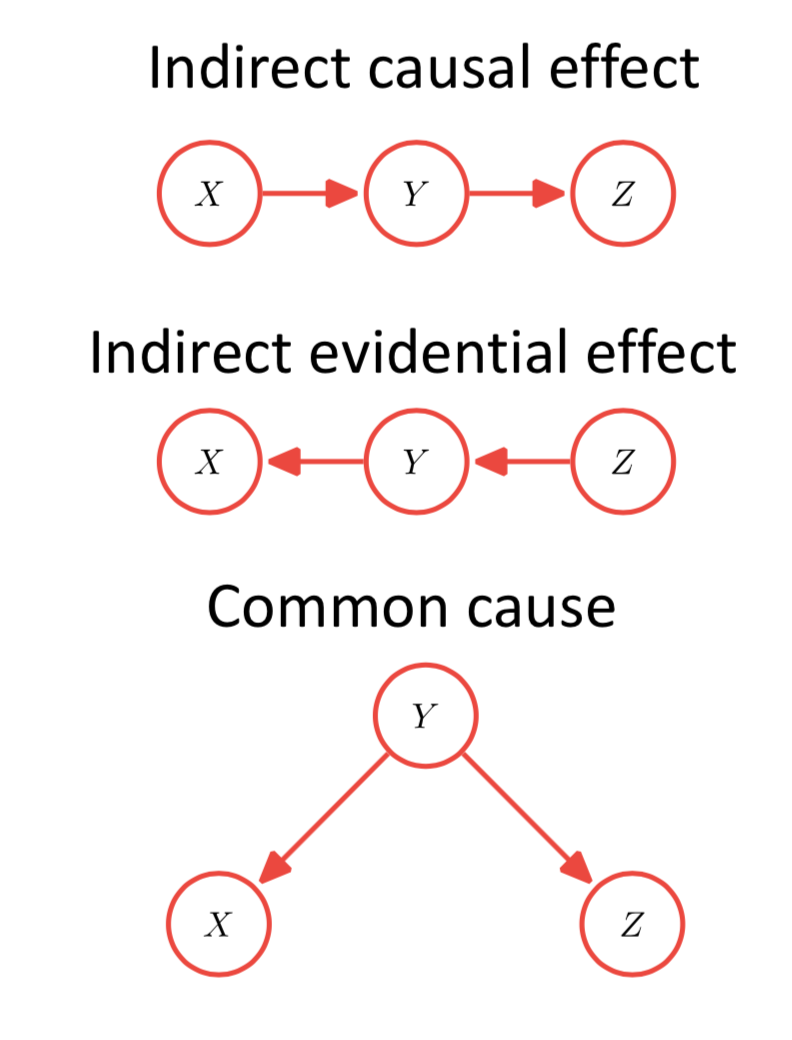
\includegraphics[scale=.2]{BN1.png}
% 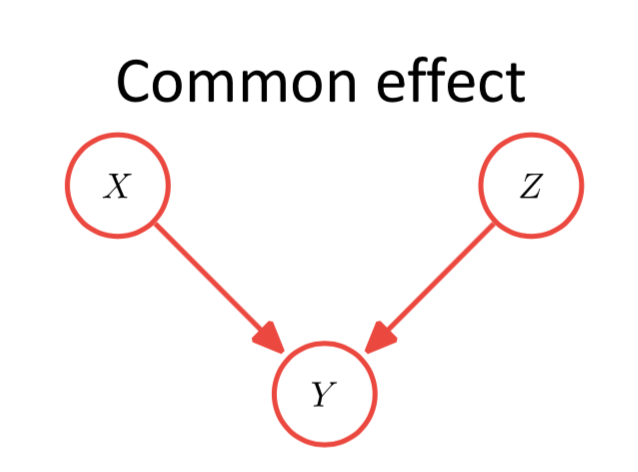
\includegraphics[scale=.2]{BN2.png}
\subsection{Active trails and d-separation}
An undirected path in a BN structure G is called active trail for observed variables $O \in {X_1, ..., X_n}$ of for every consecutive triple of variables X, Y, Z on the path:\\
- \textbf{indirect causal effect}:\\
$X \rightarrow Y \rightarrow Z$ and Y unobserved\\
- \textbf{indirect evidential effect}:\\
$X \leftarrow Y \leftarrow Z$ and Y unobserved\\
- \textbf{common cause}:\\
$X \leftarrow Y \rightarrow Z$ and Y unobserved.\\
- \textbf{common effect}:\\
$X \rightarrow Y \leftarrow Z$ and Y or any of Y's descendants is observed.\\
Any variables $X_i$ and $X_j$ for which there is no active trail for observations O are called d-separated by O.\\
\textbf{Theorem}: $d-sep(X_i;X_j|O)) \quad \Rightarrow X\perp Y |Z$\\
Converse does not hold in general!


\section{Exact inference (tree-structured BN) }
\subsection{Variable elimination}
- Given a BN and query $P(X|E=e)$\\
- Choose an ordering of $X_1, ..., X_n$ \textbf{Eliminate variables from the outside in!}\\
- Set up initial factors: $f_i=P(X_i|Pa_i)$\\
- For $i=1:n, X_i \notin {X, E}$\\
$\quad$ - Collect and multiply all factors $f$ that include $X_i$\\
$\quad$ - Generate new factor by marginalizing out $X_i$:
        $g_X_i = \sum_{x_i}\prod_j f_j$\\
$\quad$ - Add g to set of factors\\
- Renormalize $P(x,e)$ to get $P(x|e)$

\textbf{Variable elimination for polytrees:}\\
- Pick a root, (avoiding $X$ and $E$)\\
- Orient edges towards root\\
- Eliminate variables according to topological order


\subsection{Avoiding recomputation: factor graphs}
FG for a BN is a bipartite graph consisting of variables (circles) and factors (rectangles). \textbf{It is not a unique representation.}\\
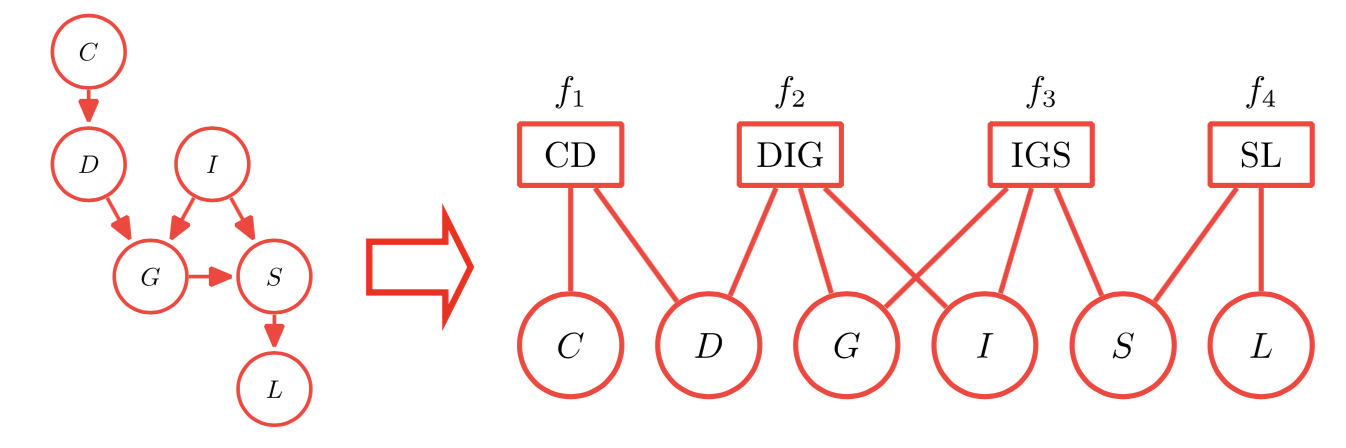
\includegraphics[scale=0.25]{images/factor_graph.png}
\subsubsection{Sum-product/Belief Propagation (BP) Algorithm:}
- Initialize all messages as uniform distribution\\
- Until converged to:\\
$\quad$ - Pick a root in the factor graph and reorient the edges towards this root.\\
$\quad$ -  Update messages according to this ordering. Do passes from leaves to root and from root to leaves.\\
- If a leaf node is a variable node: 
$\mu_{x\rightarrow f}(x)=1$
- If a leaf node is a factor node:
$\mu_{f \rightarrow x}(x)=f(x)$
- Messages from node $v$ to factor $u$:\\
    $\mu_{v\rightarrow u}(x_v) = \prod_{u'\in N(v)\setminus \{u\}}\mu_{u'\rightarrow v(x_v)}$\\
- Messages from factor $u$ to node $v$:\\
    $\mu_{u\rightarrow v}(x_v) = \sum_{x_u\sim x_v}f_u(x_u) \prod_{v'\in N(u)\setminus \{v\}}\mu_{v'\rightarrow u(x_v')}$
    % https://tex.stackexchange.com/questions/9363/how-does-one-insert-a-backslash-or-a-tilde-into-latex
$\quad$ -  Break once all messages change by $\leq \epsilon$

\textbf{Hope:} after convergence, we have:\\
$P(X_v=x_v)=\frac{1}{Z}\prod_{u \in N(v)}\mu_{u\rightarrow v}(x_v)$\\
$P(\overrightarrow{X_u}=\overrightarrow{x_u})=\frac{1}{Z} f_u(\overrightarrow{x_u})\prod_{v\in N(u)}\mu_{v\rightarrow u}(x_v)$

\textbf{If we have a polytree Bayesian network}:\\
- Choose one node as root\\
- Send messages from leaves to root and from root to leaves\\


\section{Approximate inference (loopy networks)}
With loopy graphs, BP is often \textbf{overconfident/oscillates}.
\subsection{Variable elimination for MPE (most probable explanation):}

- Given BN and evidence E=e\\
- Choose an ordering of $X_1, ... x_n$\\
- Set up initial factors $f_i=P(X_i|Pa_i)$\\
- For $i=1:n, X_i \notin  E$:\\
$\quad$ - Collect and multiply all factors $f_j$ that include $X_i$\\
$\quad$ - Generate new factor by maximizing out $X_i$:
        $g_i=\underset{w=x_i}{\operatorname{max}}\prod_j f_j$\\
$\quad$ - Add $g$ to set of factors\\
- For $i=n-1:1, X_i\notin E$:
    $\hat{x}_i=\underset{x_i}{\operatorname{argmax}}g_i(x_i, \hat{x}_{i+1:n})$

\textbf{Retrieving MAP from Max-Product (MAP = MPE for a subset of RVs):}\\
- Define max-marginals:\\
    $P_{max}(X_v=x_v):=\underset{x\sim x_v}{\operatorname{max}}P(x)$\\
- For tree factor graphs, max-product computes max-marginals:\\
    $P_{max}(X_v=x_v)	\propto \prod_{u \in N(v)} \mu_{u \rightarrow v}(x_v)$\\
- Can retrieve MAP solution from these (must be careful when ties need to be broken).


\subsection{Sampling based inference: compute marginals as expectations}
\textbf{Hoeffding's inequality:} Suppose $f$ is bounded in $[0, C]$. Then:\\
$P(|E_P[f(X)]-\frac{1}{N}\sum_{i=1}^N f(x_i)|\geq\epsilon) \leq 2exp\big( \frac{-2N\epsilon^2}{C^2}\big)$

\textbf{Monte Carlo Sampling from a BN:}\\
- Sort variables in topological ordering $X_1, X_n$\\
- For $i=1$ to $n$, sample:\\
$x_i \sim P(X_1=x_1, ..., X_{i-1}=x_{i-1})$

\textbf{Rejection Sampling}:\\
- Collect samples over all variables:\\
    $\hat{P}(X_A =x+A | X_B=x_B)=\frac{Count(x_A, x_B)}{Count(x_B)}$\\
- Throw away samples that disagree with $x_B$\\
- Count fraction of $x_a$ on remaining samples


\subsubsection{Directly sampling from the posterior: MCMC}
\textbf{Markov Chain:}: A (stationary) MC is a sequence of RVs $X_1, ..., X_N$, with prior $P(X_1)$ and transition probabilities $P(X_{t+1}|X_t)$ independent of t.\\
\textbf{Markov assumpt.:} $X_{1:t-1}\perp X_{t+1:T}|X_t$, $\forall t>1$\\
\textbf{Stationarity assumption:}\\
$P(X_{t+1}=x|X_t=x')=P(X_{t}=x|X_{t-1}=x')$, $\forall t>1$\\
\textbf{If ergodic} (= there exists a finite t such that every state can be reached in exactly t steps), then: it has a unique and positive stationary distribution $\pi(X)>0$, such for all $x$:\\
            $\underset{N\rightarrow\infty}{lim}P(X_N=x)=\pi(x)$ and $\pi(X)\perp P(X_1)$.\\
If MC satisfies the \textbf{detailed balance equation} (for unnormalized distribution $Q$, for all $x,x'$: $Q(x)P(x'|x)=Q(x')P(x|x')$), then the MC has stationarity distribution $\pi(X)=1/ZQ(X)$.

\textbf{Designing Markov Chains:}\\
- Proposal distribution $R(X'|X)$: given $X_t=x$, sample "proposal" $x'\sim R(X'|X=x)$\\
- Acceptance distribution\\
$\quad$ - Suppose $X_t=x$\\
$\quad$ - With probability $\alpha=min \Big\{1, \frac{Q(x')R(x|x')}{Q(x)R(x'|x)}\Big\}$
        set: $X_{t+1}=x'$\\
$\quad$ - With probability $1-\alpha$, set $X_{t+1}=x$\\

\textbf{MCMC for graphical models: Gibbs sampling (Random Vs \hl{Practical variant}):}\\
- Start with initial assignment $x$ to all variables\\
- Fix observed variables $X_B=x_B$\\
- For $t=1$ to $\infty$, do:\\
$\quad$ - Pick a variable $i$ uniformly at random from $\{1,...,n\}\setminus B$ \hl{/ Set ordering}, and then, for each $X_i$ (except those in $B$)\\
$\quad$ - Set $v_i=$ values of all $x$ except $x_i$\\
$\quad$ - Sample $x_i$ from $P(X_i|v_i)$





\section{Dynamical models (include time)}

\subsection{Examples with one variable per time step}
% \textbf{Hidden Markov Models (HMM)}\\
% \textbf{Kalman FIlters}\\
% 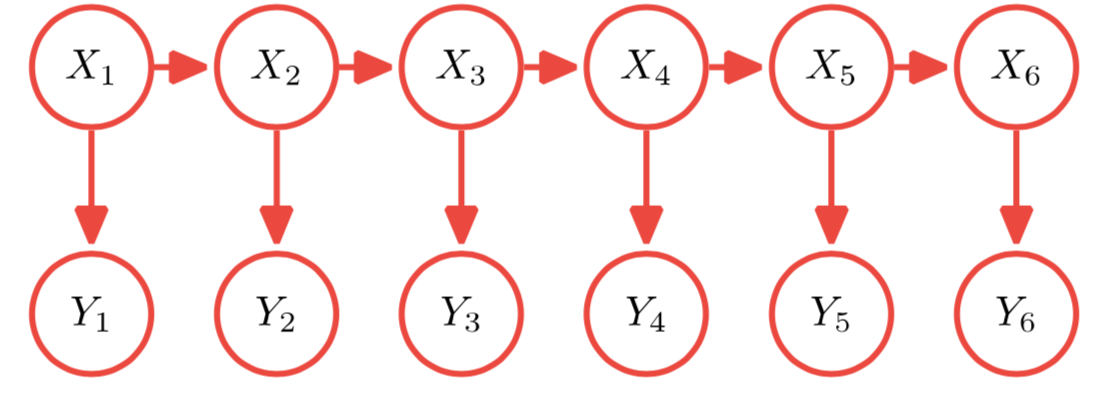
\includegraphics[scale=.25]{HMM_KF.png}\\
$X_1, ...,X_T$ (unobserved) hidden states\\
$Y_1, ...,Y_T$ (noisy) observations\\
\textbf{HMMs (polytrees: can use belief propagation):} $X_i$ categorical, $Y_i$ categorical (or arbitrary)\\
\textbf{Kalman filters:} $X_i, Y_i$ Gaussian distributions\\
- $P(X_1)$: prior belief about location at time i\\
- $P(X_{t+1}|X_t)$: \textbf{'Motion model'} (how do I expect my target to move in the environment?): 
    $X_{t+1}=FX + \epsilon_t$ where $\epsilon_t \sim N(0, \Sigma_x)$\\
- $P(Y_t|X_t)$: \textbf{'Sensor model'} (what do I observe if target is at location $X_t$?)
    $Y_t=HX_t+\eta_t$ where $\eta_t\sim N(0, \Sigma_y)$

\subsection{Inference tasks}
\textbf{Filtering}: $P(X_t|y_{1,...,t})$ Is it raining today?\\
\textbf{Prediction}: $P(X_{t+\tau}|Y_{1:t})$ Rain 5 days from now? \\
Example for one step:
$P(X_{t+1}|Y_{1:t})=\sum_x P(X_{t+1}, X_t=x_t|Y_{1:t})=\sum_x P(X_{t+1} | X_t=x_t)P(X_t|Y_{1:t})$ (with KFs, you need \textbf{integrals}!)\\
\textbf{Smoothing}: $P(X_\tau|y_{1:t})$ with $\tau<t$ Did it rain last week? [Can use sum-product (aka forward-backward).] \\
\textbf{MPE}:  $ \underset{x_{1:T}}{argmax}P(x_{1:T}|y_{1:T})$ Can use max product (aka Viterbi algorithm).\\
\textbf{Bayesian filtering:}
Start with $P(X_1)$:\\
At time t, assume we have $P(X_t|y_{1:t-1})$\\
Conditioning: 
$P(X_t|y_{1:t})= \frac{P(X_t|y_{1:t-1})P(y_t|X_t)}{\sum_{x_{t}} P(X_t|y_{1:t-1})P(y_t|X_t)}$\\
Prediction ($O(n^2)$ \textit{vs} $O(n)$ in conditioning):\\ 
$P(X_{t+1}|y_{1:t}) = \sum_x P(X_{t+1}|X_t)P(X_t|y_{1:t})$\\
\textbf{Since HMM is a polytree, smoothing/MPE can be computed by VE/BP.}
\textbf{Kalman filtering:} Bayesian filtering for continuous problems. RV corrupted by Gaussian distributions with zero mean. \textbf{Bayesian filtering is basically the same, except that sums turn to integrals.}
\textbf{General Kalman update}\\
- Transition model:
    $P(x_{t+1}|x_t)=N(x_{t+1};Fx_t, \Sigma_x)$\\
- Sensor model:
    $P(y_{t}|x_t)=N(y_{t};Hx_t, \Sigma_y)$\\
- Kalman update:\\
    $\mu_{t+1}=F\mu_t+K_{t+1}(y_{t+1}-HF\mu_t)$\\
    $\Sigma_{t+1}=(I-K_{t+1})(F\Sigma_tF^T + \Sigma_x)$\\
- Kalman gain:
    $K_{t+1}=(F\Sigma_t F^T+\Sigma_x)H^T(H(F\Sigma_t F^T+\Sigma_x)H^T+ \Sigma_y)^{-1}$


\subsection{Examples with > 1 variable per time step}
\textbf{Dynamic Bayesian Networks}: a BN at every time step\\
% 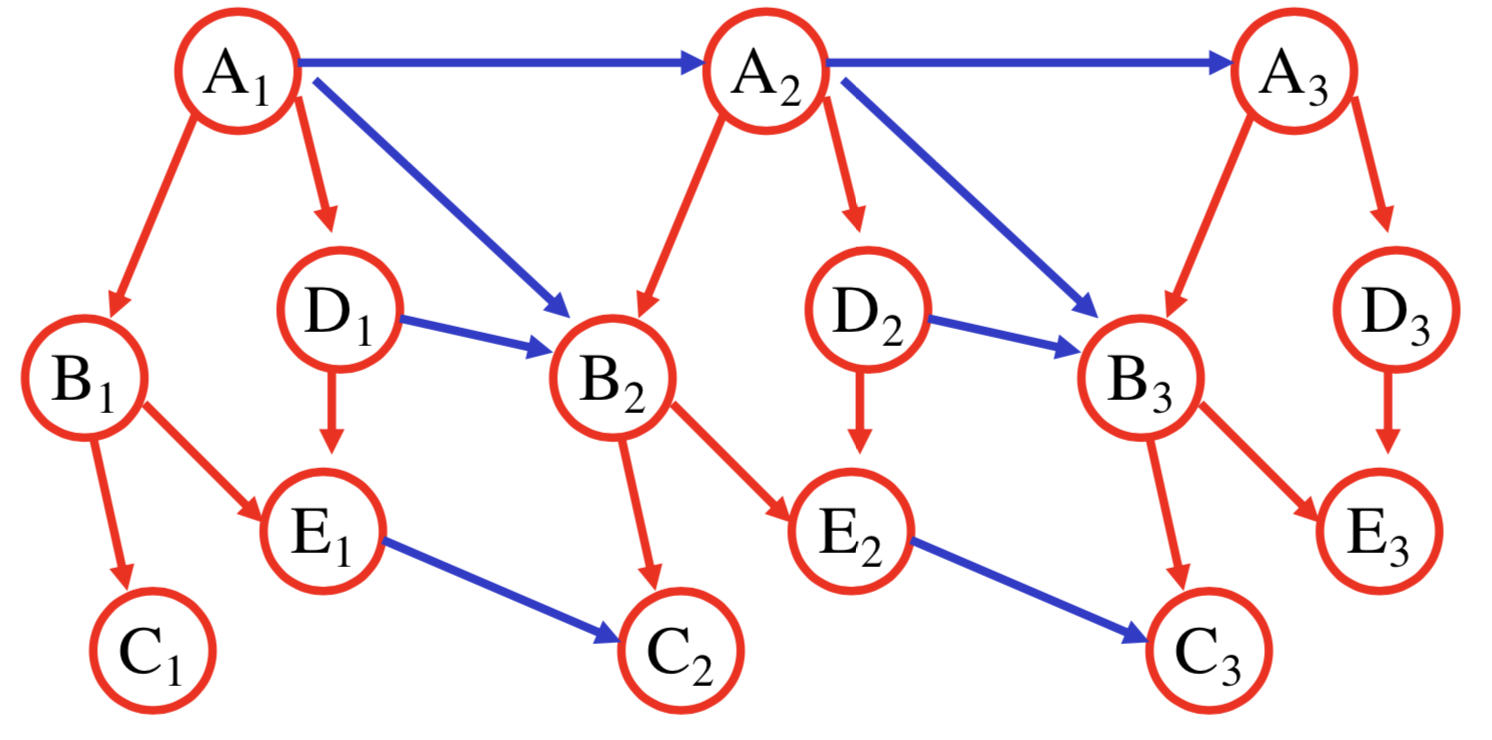
\includegraphics[scale=.1]{DBN.png}
These models typically have many loops. Exact inference is usually intractable.
\subsection{Approx. infer. for filtering (DBNs and nonlinear Kalman filters): Particle filtering}
\textbf{Suppose}: $P(X_t|y_{1:t})\approx \frac{1}{N}\sum_{i=1}^N \delta_{x_{i, t}}$, where $\delta$ is the indicator function.
\textbf{Prediction}: Propagate each particle: $x'_i \sim P(X_{t+1}|x_{i,t})$\\
\textbf{Conditioning}:\\
- weight particles $w_i=\frac{1}{Z}P(y_{t+1}|x'_i)$\\
- resample N particles $x_{i, t+1}  \sim \frac{1}{Z} \sum_{i=1}^N w_i \delta_{x'_i}$\\
% \textbf{Conclusion we came to:} $\frac{\sum_{i=1}^N w_i \delta_{x'_i}}{\sum_{i=1}^N w_i \delta_{x_i}}$
\textbf{Conclusion we came to:} $Z =\sum_{i=1}^N w_i \delta_{x_i}$

\section{Probabilistic Planning}
\subsection{Markov Decision Processes}
An MDP is specified by a quintuple: $(X, A, r, P(x'|x, a), \gamma)$, where $X$ are states, $A$ are actions, $r(x,a)$ is a reward function and transition probabilities:\\
    $P(x'|x,a)=\text{Prob(Next state}=x'|\text{Action } a)$\\ 
\textbf{Objective:} find a stationary policy $\pi: S \rightarrow A$ that maximizes the sum of cumulative rewards.
\textbf{Value of a state given a policy :} sum of cumulative rewards, given that the initial state is this state $\rightarrow$ \textbf{Bellman equation:}\\
$V^\pi(s)=\mathbb{E}\Big[ \sum_{t=0}^\infty \gamma^tr(s_t, \pi(s_t), s_{t+1})|s_0=s\Big]$\\
$= \sum_{s'\in S}P(s'|s, \pi(s))\big[r(s, \pi(s),s')+\gamma V^\pi(s')\big]$\\
$= r(s, \pi(s))+\gamma\sum_{s'\in S}P(s'|s,\pi(s))V^\pi(s')$

% 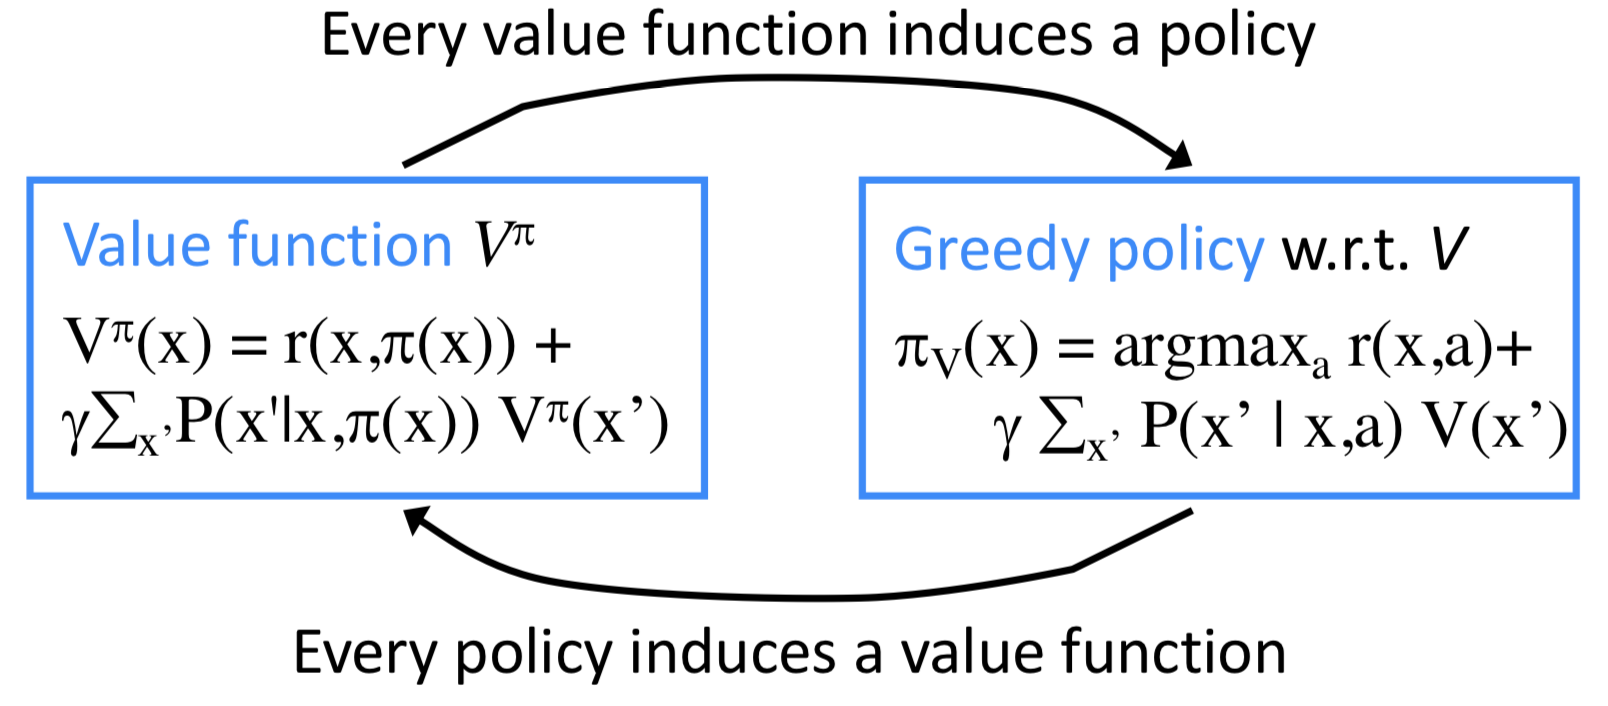
\includegraphics[scale=0.25]{valueFunctionAndPolicy.png}
\textbf{Theorem (Bellman)}: a policy is optimal iff it is greedy w.r.t. its induced value function!\\
$V^*(x)=max_a[r(x,a)+\gamma \sum_{x'}P(x'|x,a)V^*(x')]$\\
Bellman equation mais geral: \\
$V^*(x)=max_a[ \sum_{x'}P(x'|x,a)(r(a, x, x')+\gamma V^*(x')])$
Optimal policy: \\
$\pi^*(s)=\underset{a\in A}{argmax} [r(x,a)+\gamma \sum_{x'}P(x'|x,a)V^*(x')]$

\subsection{Policy iteration (Cost $O(S^3+SA\Delta)$)}
Start with an arbitrary (e.g. random) policy $\pi$.
Until converged, do:\\
- Compute value function $V^\pi (x)$\\
- Compute greedy policy $\pi_G$ w.r.t. $V^\pi$\\
- Set $\pi \leftarrow \pi_G$\\
Guaranteed to monotonically improve and to converge to an \textbf{optimal} policy $\pi^*$ in $O(n^2m/(1-\gamma))$ iterations (converges in polynomial number of iterations)!

\subsection{Value iteration (Cost $O(SA\Delta)$)}
Initialize $V_0(x)=max_a r(x,a)$\\
For $t=1$ to $\infty$:\\
- For each $(x,a)$, let: \\
$Q_t(x,a)=r(x,a)+\gamma\sum_{x'}P(x'|x,a)V_{t-1}(x')$\\
- For each $x$, let $V_t(x)=\underset{a}{max}Q_t(x,a)$\\
- Break if $||V_t-V_{t-1}||_{\infty}=\underset{x}{max}|V_t(x)-V_{t-1}(x)|\leq\epsilon$\\
Then choose greedy policy w.r.t $V_t$.\\
Guaranteed to converge to $\epsilon$-optimal policy (finds approximate solution in polynomial number of iterations)!

\subsection{POMDP = Belief-state MDP}
States = beliefs over states for original POMDP\\
$B=\Delta({1,...,n})=\{ b:{1,...,n} \rightarrow [0,1],\sum_x b(x)=1 \}$\\
Actions: same as original MDP\\
\textbf{Transition model:}\\
- Stochastic observation:\\
$P(Y_t|b_t)=\sum_{x=1}^n P(Y_t|X_t=x)b_t(x)$\\
- State update (Bayesian filtering!), given $b_t, y_t, a_t$:
$b_{t+1}(x')=\frac{1}{Z}\sum_xb_t(x)P(y_t|x)P(X_{t+1}=x'|X_t=x,a_t)$\\
Reward function: $r(b_t, a_t)=\sum_x b_t(x)r(x,a_t)$

\subsection{Example of approx. solution to POMDPs: Policy gradients}
- Assume parameterized policy: $\pi(b)=\pi(b;\theta)$\\
- For each parameter $\theta$ the policy induces a Markov chain\\
- Can compute expected reward $J(\theta)$ by sampling.\\
- Find optimal parameters through search (gradient ascent):
$\theta^* = \underset{\theta}{arg max}\quad J(\theta)$



\section{Learning models from training data}
\subsection{Learning from i.i.d data}
\textbf{Algorithm for Bayes Net MLE}:\\
Given BN of structure G and dataset D of complete observations\\
For each $X_i$ estimate:
$\hat{\theta}_{X_i|Pa_i}=\frac{Count(X_i, Pa_i)}{Count(Pa_i)}$\\
Pseudo-counts for lime and cherry flavor: $\theta_{F=c}\frac{Count(F=c)+\alpha_c}{N+\alpha_c + \alpha_l}$

\subsubsection{Score based structure learning}
Define scoring function $S(G;D)$ and search over BN structure G: $G^*=\underset{G}{argmax}S(G;D)$\\
\textbf{Examples of scores:\\
MLE Score}:\\
$log P(D|\theta_G, G) = N \sum_{i=1}^n \hat{I}(X_i;Pa_i) + const.$\\
\textbf{Where mutual information} ($I(X_i, X_j)\geq 0$) is:\\
$I(X_i, X_j)=\sum_{x_i, x_j}P(x_i, x_j)log\frac{P(x_i, x_j)}{P(x_i)P(x_j)}$ \\
\textbf{Empirical mutual information:}\\
$\hat{P}(x_i,x_j)=\frac{Count(x_i, x_j)}{N}$\\
$\hat{I}(X_i, X_j)= \sum_{x_i, x_j}\hat{P}(x_i, x_j)log\frac{\hat{P}(x_i, x_j)}{\hat{P}(x_i)\hat{P}(x_j)}$\\
\textbf{Regularizing a Bayes Net:}\\
$S_{BIC}(G) = \sum_{i=1}^n \hat{I}(X_i;Pa_i) - \frac{log N}{2N}|G|$ \\
where $G$ is the number of parameters, $n$ the number of variables and $N$ the number of training examples.\\
\textbf{Chow-Liu algorithm:}\\
- For each pair $X_i, X_j$ of variables, compute: $\hat{P}(x_i,x_j)=\frac{Count(x_i, x_j)}{N}$\\
- Compute mutual information\\
- Define complete graph with weight of edge $(X_i, X_j)$ given by the mutual information\\
- Find max spanning tree $\rightarrow$ undirected tree\\
- Pick any variable as root and orient the edges away using breadth-first search.\\


\section{Reinforcement Learning}

\subsection{Model-based RL}

\subsubsection{$\epsilon$ greedy}
With probability $\epsilon$, pick random action. With prob $(1-\epsilon)$, pick best action. If sequence $\epsilon$ satisfies Robbins Monro criteria $\rightarrow$ convergence to optimal policy with prob 1.

\subsubsection{$R_{max}$ algorithm}
\textbf{Input}: starting $x_0$, discount factor $\gamma$.\\
\textbf{Initially}: add fairy tale state $x^*$ to MDP\\
- Set $r(x,a)=R_{max}$ for all states x and actions $a$\\
- Set $P(x^*|x,a)=1$ for all states $x$ and actions $a$\\
- Choose the optimal policy for $r$ and $P$\\
\textbf{Repeat}:
1. Execute policy $\pi$ and, for each visited state/action pair, update $r(x,a)$\\
2. Estimate transition probabilities $P(x^{'}|x,a)$\\
3. If observed 'enough' transitions/rewards, recompute policy $\pi$, according to current model $P$ and $r$.\\
\textbf{"Enough"?} See Hoeffding's inequality. To reduce error $\epsilon$, need more samples $N$.\\
\textbf{Theorem}: With probability $1-\delta$, $R_{max}$ will reach an $\epsilon$-optimal policy in a number of steps that is polynomial in $|X|, |A|, T, 1/\epsilon$ and $log(1/\delta)$. Memory $O(|X^2||A|)$. 

\subsection{Model-free RL: estimate V*(x) directly}
\subsubsection{Q-learning}
$Q(x,a) \leftarrow (1-\alpha_t)Q(x,a) + \alpha_t(r+\gamma \max_{a'}Q(x', a'))$\\
% $V^*(x)=\underset{a}{max}Q*(x,a)$\\
\textbf{Theorem}: If learning rate $\alpha_t$ satisfies: $\sum_t \alpha_t=\infty$ and $\sum_t \alpha_t^2 < \infty$ (Robbins-Monro), and actions are chosen at random, then $Q$ learning converges to optimal $Q^*$ with probability 1.\\
\textbf{Optimistic Q learning:}\\
Initialize: $Q(x,a)=\frac{R_{max}}{1-\gamma}\prod_{t=1}^{T_{init}}(1-\alpha_t)^{-1}$\\
Same convergence time as with $R_{max}$. Memory $O(|X||A|)$. Comp: $O(|A|)$.\\
\textbf{Parametric Q-function approximation}: $Q(x,a;\theta)=\theto^T\phi (x,a)$ to scale to large state spaces. (You can use Deep NN here!)\\
\textbf{SGD for ANNs}: initialize weights. For t = 1,2..., pick a data point (x,y) uniformly at random. Take step in negative gradient direction. (In practise, mini-batches).\\
\textbf{Deep Q Networks}: use CNN to approx Q function.
% Use "experience relay". Clone network to maintain constant "target" values across episodes:
$ L(\theta)=\sum_{(x,a,r,x')\in D}(r+\gamma\underset{a'}{max}Q(x',a';\theto^{old})-Q(x,a;\theto))^2$ \textbf{Double DQN:} current network for evaluating argmax (too optimistic, and you remove $\theta^{old}$ and put $\theta$).

\subsection{Gaussian processes}
A GP is an (infinite) set of random variables (RV), indexed by some set X, i.e., for each x in X, there is a RV $Y_x$ where there exists functions $\mu : X \rightarrow \mathbb{R}$ and $K: X \times X \rightarrow \mathbb{R}$ such that for all: $A \in X, \quad A={x_1,...x_k}$, it holds that $Y_A=[Y_{x_1},...,Y_{x_k}] \sim N(\mu_a, \Sigma_{AA})$, where: $\Sigma_{AA} =$ matrix with all combinations of $K(x_i, x_j)$.
% \[ 
% \left (
%   \begin{tabular}{cccc}
%   K(x_1,x_1) & K(x_1,x_2) & \cdots & K(x_1,x_n) \\
%   \vdots &  &  & \vdots \\
%   K(x_k,x_1) & K(x_k,x_2) & \cdots &K(x_k,x_k)
%   \end{tabular}
% \right )
% \]

% $\mu_A =$\begin{pmatrix}\mu(x_1)\\\mu(x_2)\\\vdots\\\mu(x_k}\end{pmatrix}
K is called kernel (covariance) function (must be symmetric and pd) and $\mu$ is called mean function.
\textbf{Making prediction with GPs:} Suppose $P(f)=GP(f;\mu, K)$ and we observe $y_i=f(\overrightarrow{x_i})+\epsilon_i$, $A=\{\overrightarrow{x_1}:\overrightarrow{x_k}\}$
$P(f(x)|\overrightarrow{x_1}:\overrightarrow{x_k},y_{1:k})=GP(f;\mu ', K')$.  In particular, $P(f(x)|\overrightarrow{x_1}:\overrightarrow{x_k},y_{1:k})=N()f(x);\mu_{x|A}, \sigma^2_{x|a}$, where $\mu_{x|a}=\mu(\overrightarrow{x})+\Sigma_{x,A}(\Sigma_{AA}+\sigma^2I)^{-1}\Sigma^T_{x,A}(\overrightarrow{y_A}-\mu_A)$ and $\sigma^2_{x|a}=K(\overrightarrow{x},\overrightarrow{x})-\Sigma_{x,A}(\Sigma_{AA}+\sigma^2I)^{-1}\Sigma^T_{x,A}$. \textbf{Closed form formulas for prediction!}






\end{multicols*}
\end{document}